\chapter{Requirement Specification}
\section{Introduction}
This part of the document outlines the requirement specification of the game Proximity Assault which will serve as the blueprint or the base for the features, functionality and quality of the game. The aim of clearly defining these requirements is to keep everyone including developers, designers, testers and even the lovely audience to be on the same page, leading to a successful development journey.
\section{Functional Requirements}
\subsection{Main Gameplay}
\begin{itemize}
\item	Player controls a character.
\item 	Levels filled with different enemies.
\item 	Player uses different weapons and tools to eliminate enemies
\end{itemize}
\subsection{Progression}
\begin{itemize}
	\item 	Unlock new game level with experience or in-game currency.
	\item 	Difficulty increases with every new level.
	\item	Optional side objectives to make the game more engaging (Optional).
\end{itemize}
\subsection{Inventory and Upgrades}
\begin{itemize}
	\item 	Player can use different weapons and tools with different attributes.
	\item 	Option to upgrade weapons for improving power and efficiency.
	\item 	Able to use some special abilities in the game.
\end{itemize}
\subsection{Menus and UI}
\begin{itemize}
	\item	Feature an extremely smooth and easy User interface for the players.
	\item 	Pause menus with options to save, quite or adjust setting of the game.
	\item 	Health bar, objective status indicator and other elements for feedback.
\end{itemize}

\section{Non-Functional}
The non-functional requirements of the system are about how a system should behave instead of what specific function to perform.
\subsection{Performance}
\begin{itemize}
	\item 	Maintain smooth frame rate and responsiveness on target platforms (iOS, Android).
	\item`	Optimize every feature in order to avoid performance issues.
\end{itemize}
\subsection{Graphics And Audio}
\begin{itemize}
	\item   Make sure the frame rate does not fall and is stable \cite {singh2023effect}
	\item 	Good sounds and background music.
	\item 	Sounds that inform the user about the certain actions enemy response fire.
\end{itemize}
\subsection{Controls}
\begin{itemize}
	\item 	Responsive and faster controls for aiming, and interacting with the environment..
	\item 	Sufficient options for customization.
\end{itemize}
\subsection{User Interface}
\begin{itemize}
	\item 	New game, continue game, exit.
	\item 	Links to social media platforms.
	\item 	Setting button to adjust controls.
\end{itemize}
\section{UI Requirements}
This includes the guidelines for how a game user interface should look and function when the player is interacting with the system. It includes menus, buttons, maps, inventory screen and health bar.
\subsection{Main menus}
\begin{itemize}
	\item	Start game, continue game, and option buttons.
	\item	Information about the game and social links.
\end{itemize}
\subsection{Gameplay Screen}
\begin{itemize}
	\item 	Health bar, Objectives status indicators, ammo/resources indicators.
	\item 	Mini map or level overview (Optional).
	\item 	Button to access inventory.
\end{itemize}
\subsection{Inventory Screen}
\begin{itemize}
	\item	Display of the available resources.
	\item 	Upgrade options with cost and description.
	\item 	Special abilities management with usage indicators.
\end{itemize}
\subsection{Pause menu}
\begin{itemize}
	\item 	Options to save, resume, quit and adjust game settings.
	\item 	Control layout and settings overview.
\end{itemize}

\section{Persona}
The Operation Bio-Purge has a very simple persona in which a user named Ali, the Casual Gamer.
\subsection{Demographics}
\begin{itemize}
	\item 	Name: Ali
	\item 	Age: 23
	\item 	Occupation: Marketing Specialist
	\item   Location: Peshawar City
	\item 	Device: IPhone 11
\end{itemize}
\subsection{Gaming Habits}
\begin{itemize}
	\item 	Play mobile game in short breaks or during free time.
	\item 	Play games with light heart themes and great visuals.
\end{itemize}
\subsection{Motivation}
\begin{itemize}
	\item For relaxing himself and enjoying in free time.
	\item 	Enjoys the satisfaction of completing short objectives.
	\item 	Like good game designs.
\end{itemize}
\subsection{Concerns}
\begin{itemize}
	\item 	Limited time to play the game
	\item	Dislike ads and in-game pop-ups for purchases or any sort of disturbance.
	\item	Do not like repetitive game play.
\end{itemize}


\section{User Interactions with the System through Use Case Diagram}
A use case diagram describes all the functionalities of the system along with external users aiming to describe how an actor (user) interacts with the system.
A use case diagram also specifies the main functionalities of the system that a user can perform while interacting with the system.The testing phase also uses the use case diagram as a base.\\
\\

\begin{figure}[H]
	\centering
	\graphicspath{./Latex Thesis}
	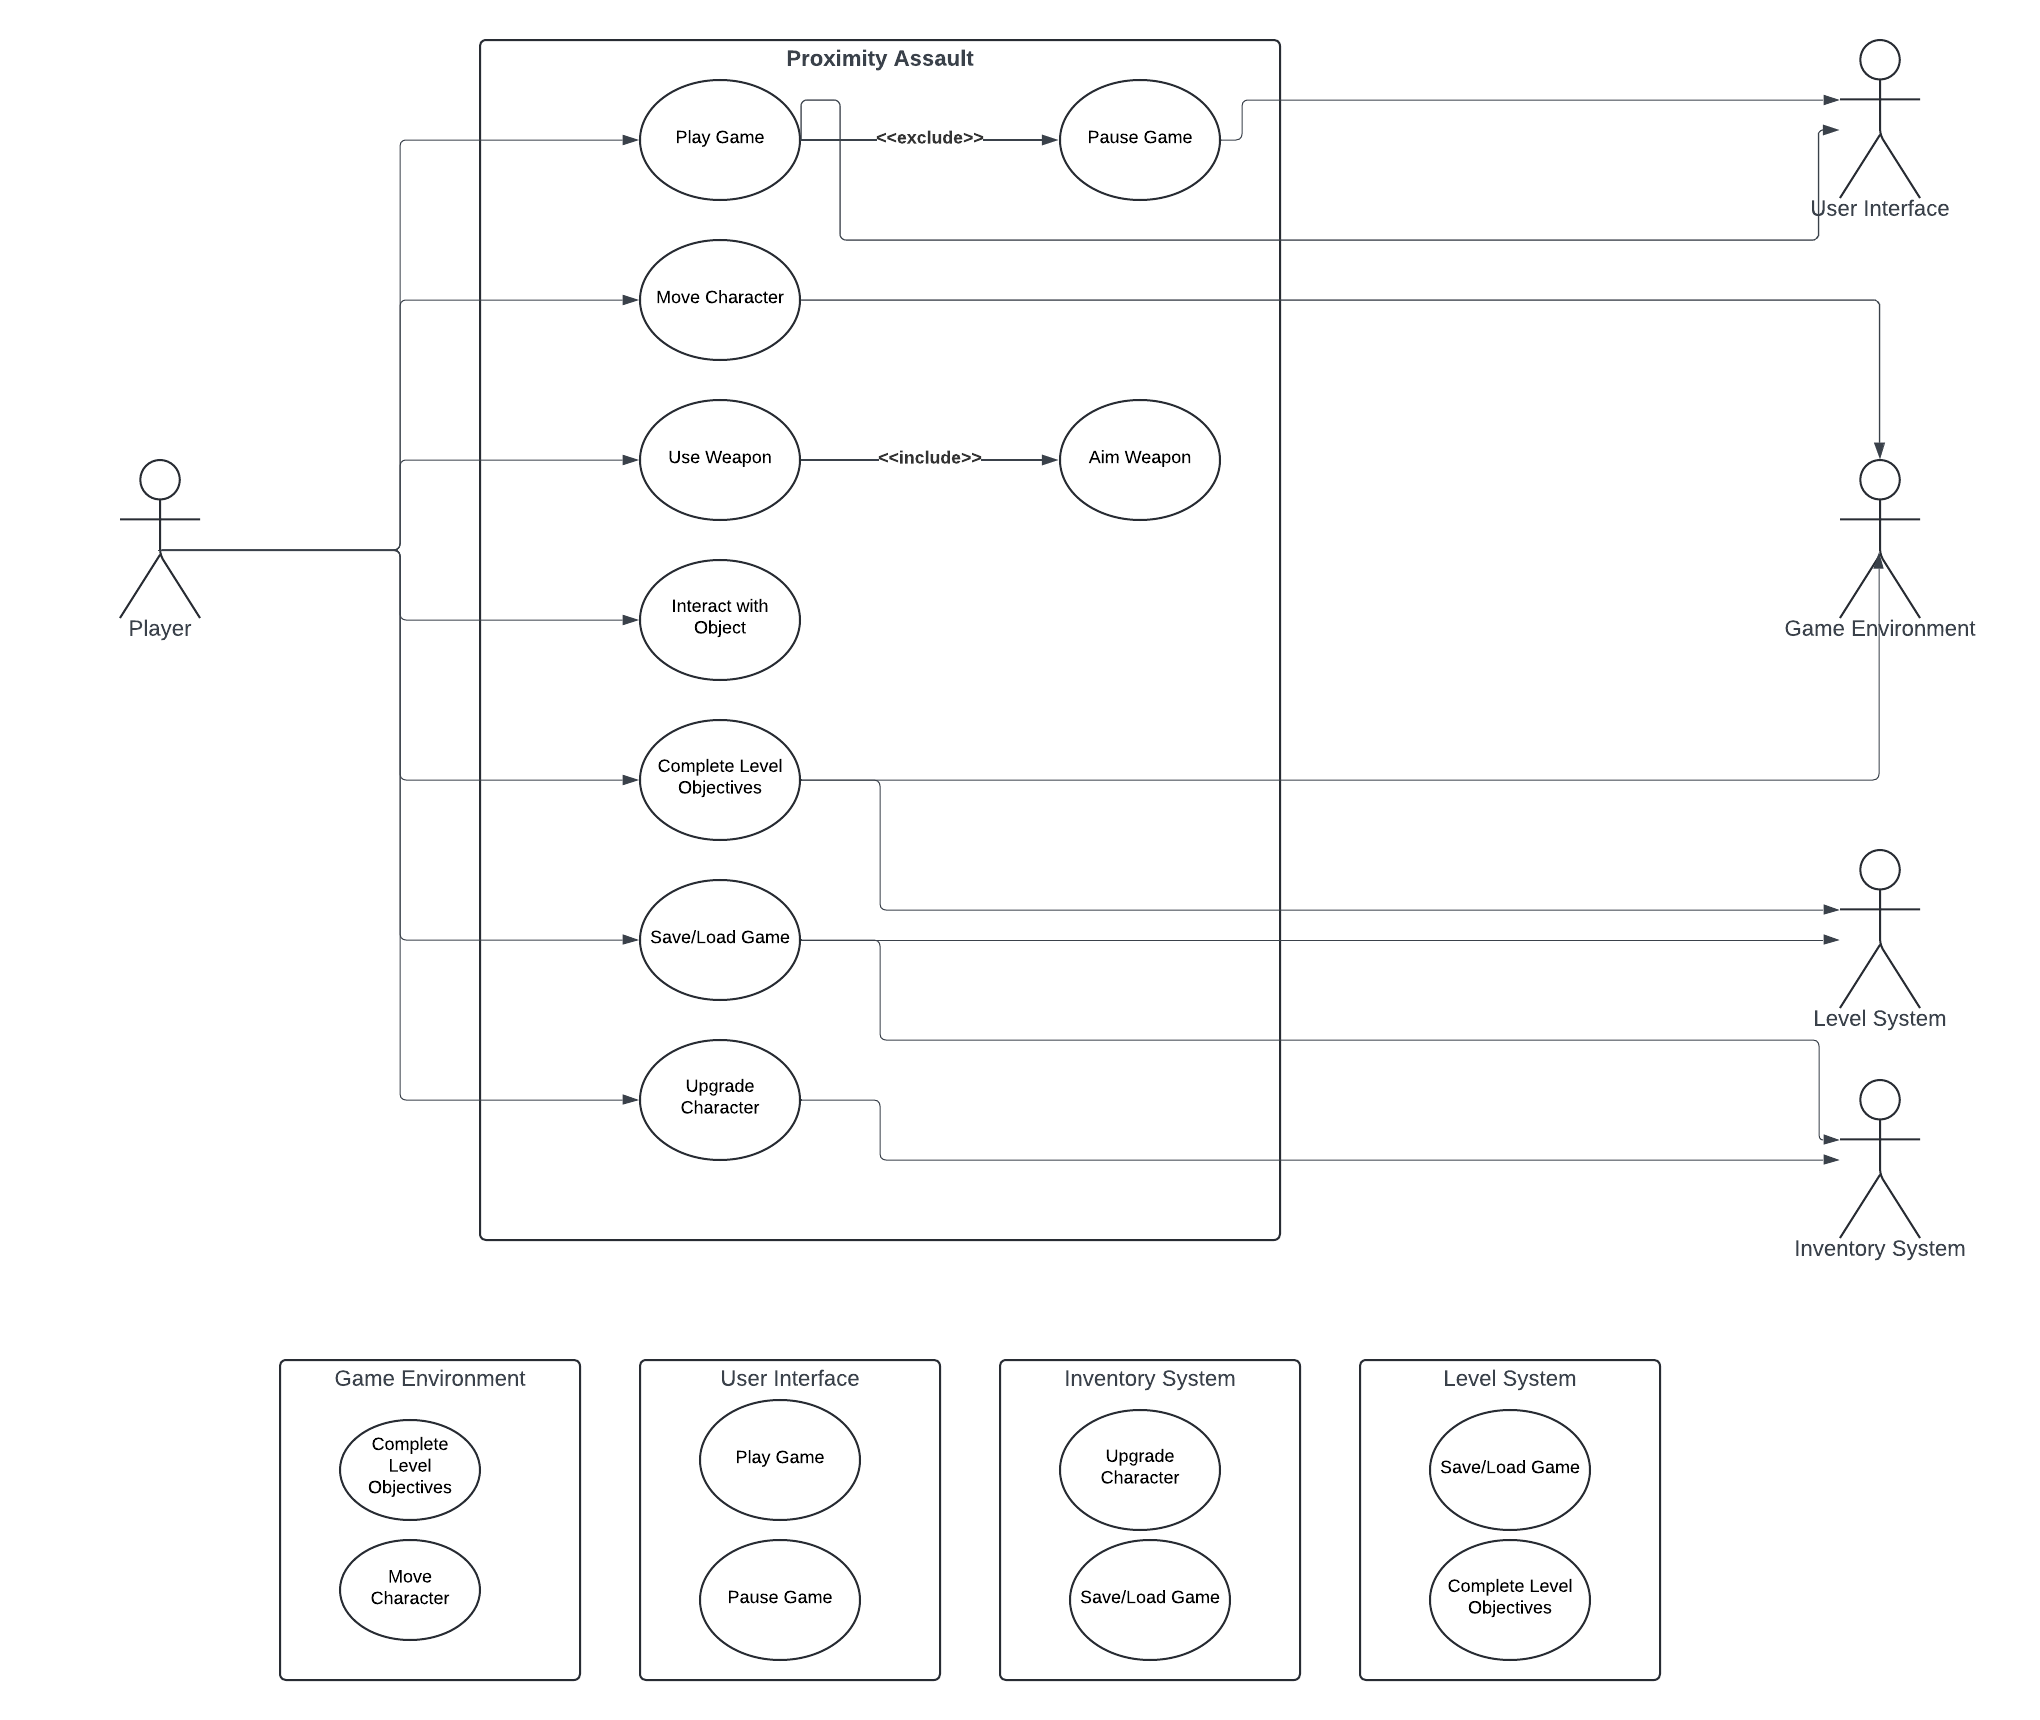
\includegraphics[width=16cm,height=12cm]{ucdiagram.png}
	\caption{Use Case Diagram for Proximity Assault.}
	\label{fig:Use Case Diagram}
\end{figure}

\section{System Boundary}
\begin{itemize}
	\item \textbf{Actor(Player):}The player represents the user interacting with the system.
	\item \textbf{Game Environment:}This represents the virtual environment where the game takes place including elements like terrains, enemies and objects.
	\item \textbf{Inventory System:} Manages the player inventory, the items that a player collects during the game play or purchases them from a store.
	\item \textbf{Level System:} This functionality manages the progression and objectives with in each level.
	\item \textbf{User Interface:}	 Provides the visual and interactive way through which a user interacts with the game.
\end{itemize}

\subsection{Use Case}
The use case describes various actions or functionalities that a player can perform while interacting with the system.
\begin{itemize}
	\item \textbf{Play Game:} Begins the game play.
	\item \textbf{Move Character:} Allows the player to move their character with in the game environment.
	\item \textbf{Interact with Object:} Enables the player to interact with objects present in the game environment.
	\item \textbf{Use Weapons/Tools:} Allows the player to utilize weapons or tools.
	\item \textbf{Collect Item (Planned):} Able to collect game items found with in the game environment.
	\item \textbf{Upgrade Character (Planned):} For Upgrading the character abilities.
	\item \textbf{Complete Level Objectives:} Indicates the accomplishment of objectives.
	\item \textbf{Save Game (Planned):} To Save the current progress within the game.
	\item \textbf{Load Game (Planned):} Loading the game from previous saved state.
\end{itemize}
\subsection{Include and exclude}Indicate the relationships between use cases
\begin{itemize}
	\item \textbf{Play game exclude pause game:} This means that when the player is playing the game, the pause functionality is not available.
	\item \textbf{Use Weapons/Tools includes Aim Weapons/Tools:} This signifies that aiming is a part of the process of using weapons within the game.
\end{itemize}
\subsection{Actor Use Case Relationships}
Arrows connecting actors (Player) to use cases indicate that players interact with those functionalities.
\section{Development Environment Requirements}
Development of this game involves various tools and software with their own system requirements, below is a very detailed information of the development environment required for this game.
\subsection{Development Environment}
\subsubsection{Operating System}
\begin{itemize}
	\item \textbf{Minimum:} Windows 10 64-bit (recommended latest stable version).
	\item \textbf{Alternative:} MacOs Mojave 10.14+ (recommended: latest stable version).
	\item \textbf{Justification:} Both Unity and MacOs are officially supported by Unity.
\end{itemize}
\subsection{Hardware}
\subsubsection{Processor}
\begin{itemize}
	\item \textbf{Minimum:} x86 or x64 architecture with SSE2 instruction set support(e.g. Intel core i5-4460 or AMD equivalent).
	\item \textbf{Recommended:} Newer processor with multiple cores (e.g., Intel core i7 or AMD Ryzen) for smoother performance during development and testing.
\end{itemize}
\subsubsection{RAM}
\begin{itemize}
	\item \textbf{Minimum:} 8GB
	\item \textbf{Recommended:} 16GB for multitasking and handling larger projects
\end{itemize}
\subsubsection{Graphics Card}
\begin{itemize}
	\item \textbf{Minimum:} DX10, DX11, DX12 capable (e.g., NVidia GTX 970 or AMD Radeon R9 290)
\end{itemize}
\subsubsection{Storages}
\begin{itemize}
	\item \textbf{Minimum:} 20GB available space for Unity and Project Files
	\item \textbf{Recommended:} More space depending on project size, additional tools and asset libraries.
\end{itemize}
\subsection{Software}
\subsubsection{Unity Game Engine}
\begin{itemize}
	\item Download the latest stable version that is compatible with your system.
	\item Consider Unity Personal for small projects or Unity Plus for additional features.
\end{itemize}
\subsubsection{Version Control}
\begin{itemize}
	\item Git (Recommended) with code hosted on GitHub
\end{itemize}
\subsubsection{Graphics Designing Software}
\begin{itemize}
	\item Photoshop, GIMP for creating UI elements textures  or logos.
\end{itemize}
\subsubsection{3D Modeling Software}
\begin{itemize}
\item	Blender
\end{itemize}
\subsubsection{Audio Editing}
\begin{itemize}
	\item Audacity
\end{itemize}
\subsubsection{Asset Creations}
\begin{itemize}
	\item \textbf{Asset Creation:} Asset will be used from unity market place.
\end{itemize}

\section{Minimum Hardware Requirements for Running the Game}
These are the requirements for running the Operation Bio-Purge game on Android or iOS. These are the general requirements needed for running the system.
\subsection{Android}
\begin{itemize}
	\item \textbf{Processor:} Dual-core 1.2 GHz processor (recommended: Quad-core 1.5 GHz or better)
	\item \textbf{RAM:} 1GB RAM (recommended 2GB or more)
	\item \textbf{Storage:} 500 MB free space 
	\item \textbf{Operating System:} Android 5.0 or later (recommended Android 8.0 or later).
	\item \textbf{Graphics:} Adreno 305 GPU or equivalent (recommended: Adreno 405 or later).
\end{itemize}
\subsection{iOS}
\begin{itemize}
	\item \textbf{Device:}	 iPhone 6 or later (recommended iPhone 7 or later).
	\item \textbf{Operating System:}  iOS 10 or later (recommended: iOS 12 or later).
	\item \textbf{RAM:} 1GB RAM (recommended: 2GB or more)
	\item \textbf{Storage:} 500 MB free space.	
\end{itemize}